\documentclass[10pt]{article}
\usepackage[utf8]{inputenc}
\usepackage[a4paper, total={6.4in, 8.53in}]{geometry}
\geometry{left=1.5cm, right=2.0cm, top=1.5cm, bottom=2.0cm}
\usepackage{hyperref}
\hypersetup{hidelinks, colorlinks = true, allcolors = black, pdfstartview = Fit, breaklinks = true}
\usepackage[utf8]{inputenc}
\usepackage{filecontents}
\usepackage{biblatex}
\usepackage{url}
\usepackage{amsmath, tikz, amsfonts, bbm, mathrsfs, graphicx, amssymb, amsthm, hyperref, centernot, enumerate, bbm, xcolor, lmodern, mathdots, amsfonts, graphicx, float}
\fontsize{7.0pt}{24pt}
\begin{filecontents}{mybib.bib}
@unpublished{Latex mathematical Formulas,
    title={Latex mathematical Formulas - detailed tutorial}, \\
    {\href{https://blog.csdn.net/NSJim/article/details/109045914}{https://blog.csdn.net/NSJim/article/details/109045914}},
    publisher={NSJim}, 
    year={2020}, 
    month={Oct}} 
\end{filecontents}
\bibliography{}

\title{MAT1856/APM466 Assignment 1}
\author{Minhui Yu, Student \#: 1005414151}
\date{February, 2020}

\begin{document}

\maketitle

\begin{enumerate}
    \item
    \begin{enumerate}
        \item 
            If a country's currency issuing institutions issue more money than necessary without a corresponding increase in productivity, that is, the production of goods does not increase accordingly, then due to supply and demand, more money will have to be used to buy goods, and the currency will depreciate in the international view.
        \item
            In long term part, if forward rate equals to spot rate, -- i.e spot rate does not change in long term, that is $f_{t-i,\ t}, \ s_t \ and \ 
             s_{t-i}$ in $(1 + \frac{f_{t-i,\ t}}{2})^{t-(t-i)} = \frac{(1+s_t)^t}{(1+s_{t-i})^{t-i}}$ are equal, then the yield curve will flatten. 
        \item
            Quantitative easing is similar to printing money indirectly, because when zero or near-zero interest rates are in place, the central bank buys long-term bonds, such as Treasury bonds, to flood the market with liquidity and encourage spending and borrowing. The (US) Fed provides credit support to households, small businesses and major employers, and allows unlimited purchases of TREASURIES and agency MBS on demand.
    \end{enumerate}
    \item 
        I choose "CAN 0.5 Feb.28.22", "CAN 2.75 May.31.22", "CAN 1.75 Feb.28.23", "CAN 1.5 May.31.23", "CAN 2.25 Feb.29.24", "CAN 1.5 Aug.31.24", "CAN 1.25 Feb.28.25", "CAN 0.5 Aug.31.25", "CAN 0.25 Feb.28.26", "CAN 1 Aug.31.26" and "CAN 1.25 Feb.28.27" (refers to the Canadian Government bond with a maturity in Month day, year and a coupon of c). First I choose to use the bonds with maturity 3-10 years, then I collected the data in 2022.01.10-2022.01.14 and 2022.01.17-2022.01.21. I noticed that most of the bonds have maturity 02.28-29 and 08.30-31 with 5-year term. Since we want to construct a “0-5 year” yield and spot curves with 10-11 bonds, the ideal interval for years until maturity of each bond should be: 0-0.5 year, 0.5-1, 1-1.5, \dots, 4.5-5 year and 5+ year. So I choose all the bonds with 5-year term and find that there are two missing 5-year bond in 0.5-1 and 1-1.5 year. Thus we use two 10-year bond whose maturity date are in 0-1 and 1-2 year respectively instead.
    \item
        First of all, PCA is if we have an n-dimensional data set with m data, and 2e want to reduce the dimension from the n down to k dimension. Ideally output is the data set with k dimension and m data to represent the original data set as much as possible. Let A be an n $\times$ n  covariance matrix, and we have $Ax = \lambda x \Rightarrow (A - \lambda I) x = 0$ where $\lambda$ is the eigenvalue and x is the eigenvector. The eigenvalues and the eigenvectors are the solution for the function above. $x \rightarrow y = Ax$ implies: x can be transformed to y by A. That is the eigenvector corresponding to the eigenvalue is the ideal coordinate axis, and the eigenvalue is equal to the variance of the corresponding dimension of the data in the rotated coordinates. The value of eigenvalues represents the contribution of corresponding eigenvectors to the whole matrix after orthogonalization. When we solve the eigenvalues and eigenvectors we sort the eigenvalues first. The larger the eigenvalues are, the more relevant the corresponding eigenvectors are in the data set.
\end{enumerate}


\begin{enumerate}
\setcounter{enumi}{3} 
    \item 
    \begin{enumerate}
        \item 
            This part shows the steps for YTM calculation. \\
            Recall: 
            $$
            \begin{scriptsize}
            P_n = cash \ flow_1 \times (1 + \frac{r_1}{2})^{-2 t_1} + cash \ flow_2 \times (1 + \frac{r_2}{2})^{-2 t_2} + \cdots
            \end{scriptsize}
            $$ 
            where P is the dirty price, $p_i$ is the cash flow in period $t_i$, $r(t_i)$ is the yield to maturity we want and $t_i$ is the remaining maturity from now (counted by year). \\
            Based on the bonds we selected, we use two 10-year bond instead there exists missing years until maturity: 0.5-1 and 1.5-2 year. We want to keep our thought, then we assume that they has the position in 0.5-1 year and 1.5-2 year. Nevertheless when we do calculations we need to pay attention to their real years until maturity to find their cash flow, ytm, ect. \\
            Recall: $Dirty Price: P_i = accrued \ interest + Clean \ Price = n/360 * annual \ coupon \ payment$ where n is number of days since last payment between "today" and coupon payment date. \\
            $coupon \ payment = \frac{annual \ coupon \ rate \times face \ value}{number \ of \ coupon \ payments \ per \ year}$
            $$
            Cash \ Flow_i=
            \begin{scriptsize}
            \begin{cases}
                coupon \ payment, & i<years \ until \ maturity \\
                coupon \ payment + face \ value , & i=years \ until \ maturity
            \end{cases}
            \end{scriptsize}
            $$
            Thus we have: 
            \begin{table}[H]
                \caption{Bonds’ Yield (YTM) from the selected 11 Bonds}
                \resizebox{\textwidth}{20mm}{
                \begin{tabular}{|c|c|c|c|c|c|c|c|c|c|c|} \hline
                    Years Until Maturity & 2022/01/10  & 2022/01/11  & 2022/01/12  & 2022/01/13  & 2022/01/14  & 2022/01/17  & 2022/01/18  & 2022/01/19  & 2022/01/20  & 2022/01/21  \\\hline
                    0-0.5 & 0.0036 & 0.0046 & 0.0042 & 0.0039 & 0.0047 & 0.0041 & 0.0060 & 0.0057 & 0.0054 & 0.0041 \\\hline
                    0.5-1 & 0.0052 & 0.0053 & 0.0053 & 0.0059 & 0.0059 & 0.0064 & 0.0067 & 0.0064 & 0.0067 & 0.0061 \\\hline
                    1-1.5 & 0.0096 & 0.0096 & 0.0097 & 0.0099 & 0.0100 & 0.0108 & 0.0111 & 0.0111 & 0.0110 & 0.0106 \\\hline
                    1.5-2 & 0.0102 & 0.0102 & 0.0104 & 0.0106 & 0.0108 & 0.0115 & 0.0118 & 0.0118 & 0.0118 & 0.0114 \\\hline
                    2-2.5 & 0.0117 & 0.0117 & 0.0119 & 0.0120 & 0.0121 & 0.0129 & 0.0133 & 0.0133 & 0.0133 & 0.0128 \\\hline
                    2.5-3 & 0.0129 & 0.0126 & 0.0126 & 0.0128 & 0.0130 & 0.0138 & 0.0141 & 0.0143 & 0.0142 & 0.0137 \\\hline
                    3-3.5 & 0.0138 & 0.0136 & 0.0138 & 0.0138 & 0.0142 & 0.0149 & 0.0153 & 0.0153 & 0.0153 & 0.0147 \\\hline
                    3.5-4 & 0.0145 & 0.0143 & 0.0141 & 0.0141 & 0.0144 & 0.0151 & 0.0155 & 0.0158 & 0.0157 & 0.0153 \\\hline
                    4-4.5 & 0.0147 & 0.0146 & 0.0147 & 0.0146 & 0.0149 & 0.0156 & 0.0161 & 0.0162 & 0.0162 & 0.0157 \\\hline
                    4.5-5 & 0.0152 & 0.0151 & 0.0152 & 0.0151 & 0.0153 & 0.0161 & 0.0166 & 0.0167 & 0.0166 & 0.0160 \\\hline
                    5 +   & 0.0157 & 0.0156 & 0.0157 & 0.0156 & 0.0158 & 0.0165 & 0.0171 & 0.0171 & 0.0171 & 0.0165 \\\hline
                \end{tabular}}
            \end{table}
            With the ytm in table 1 above, we can plot the yield curve now (by concatenating YTM with different years until maturity on the same date): 
            \begin{figure}[H]
                \centering
                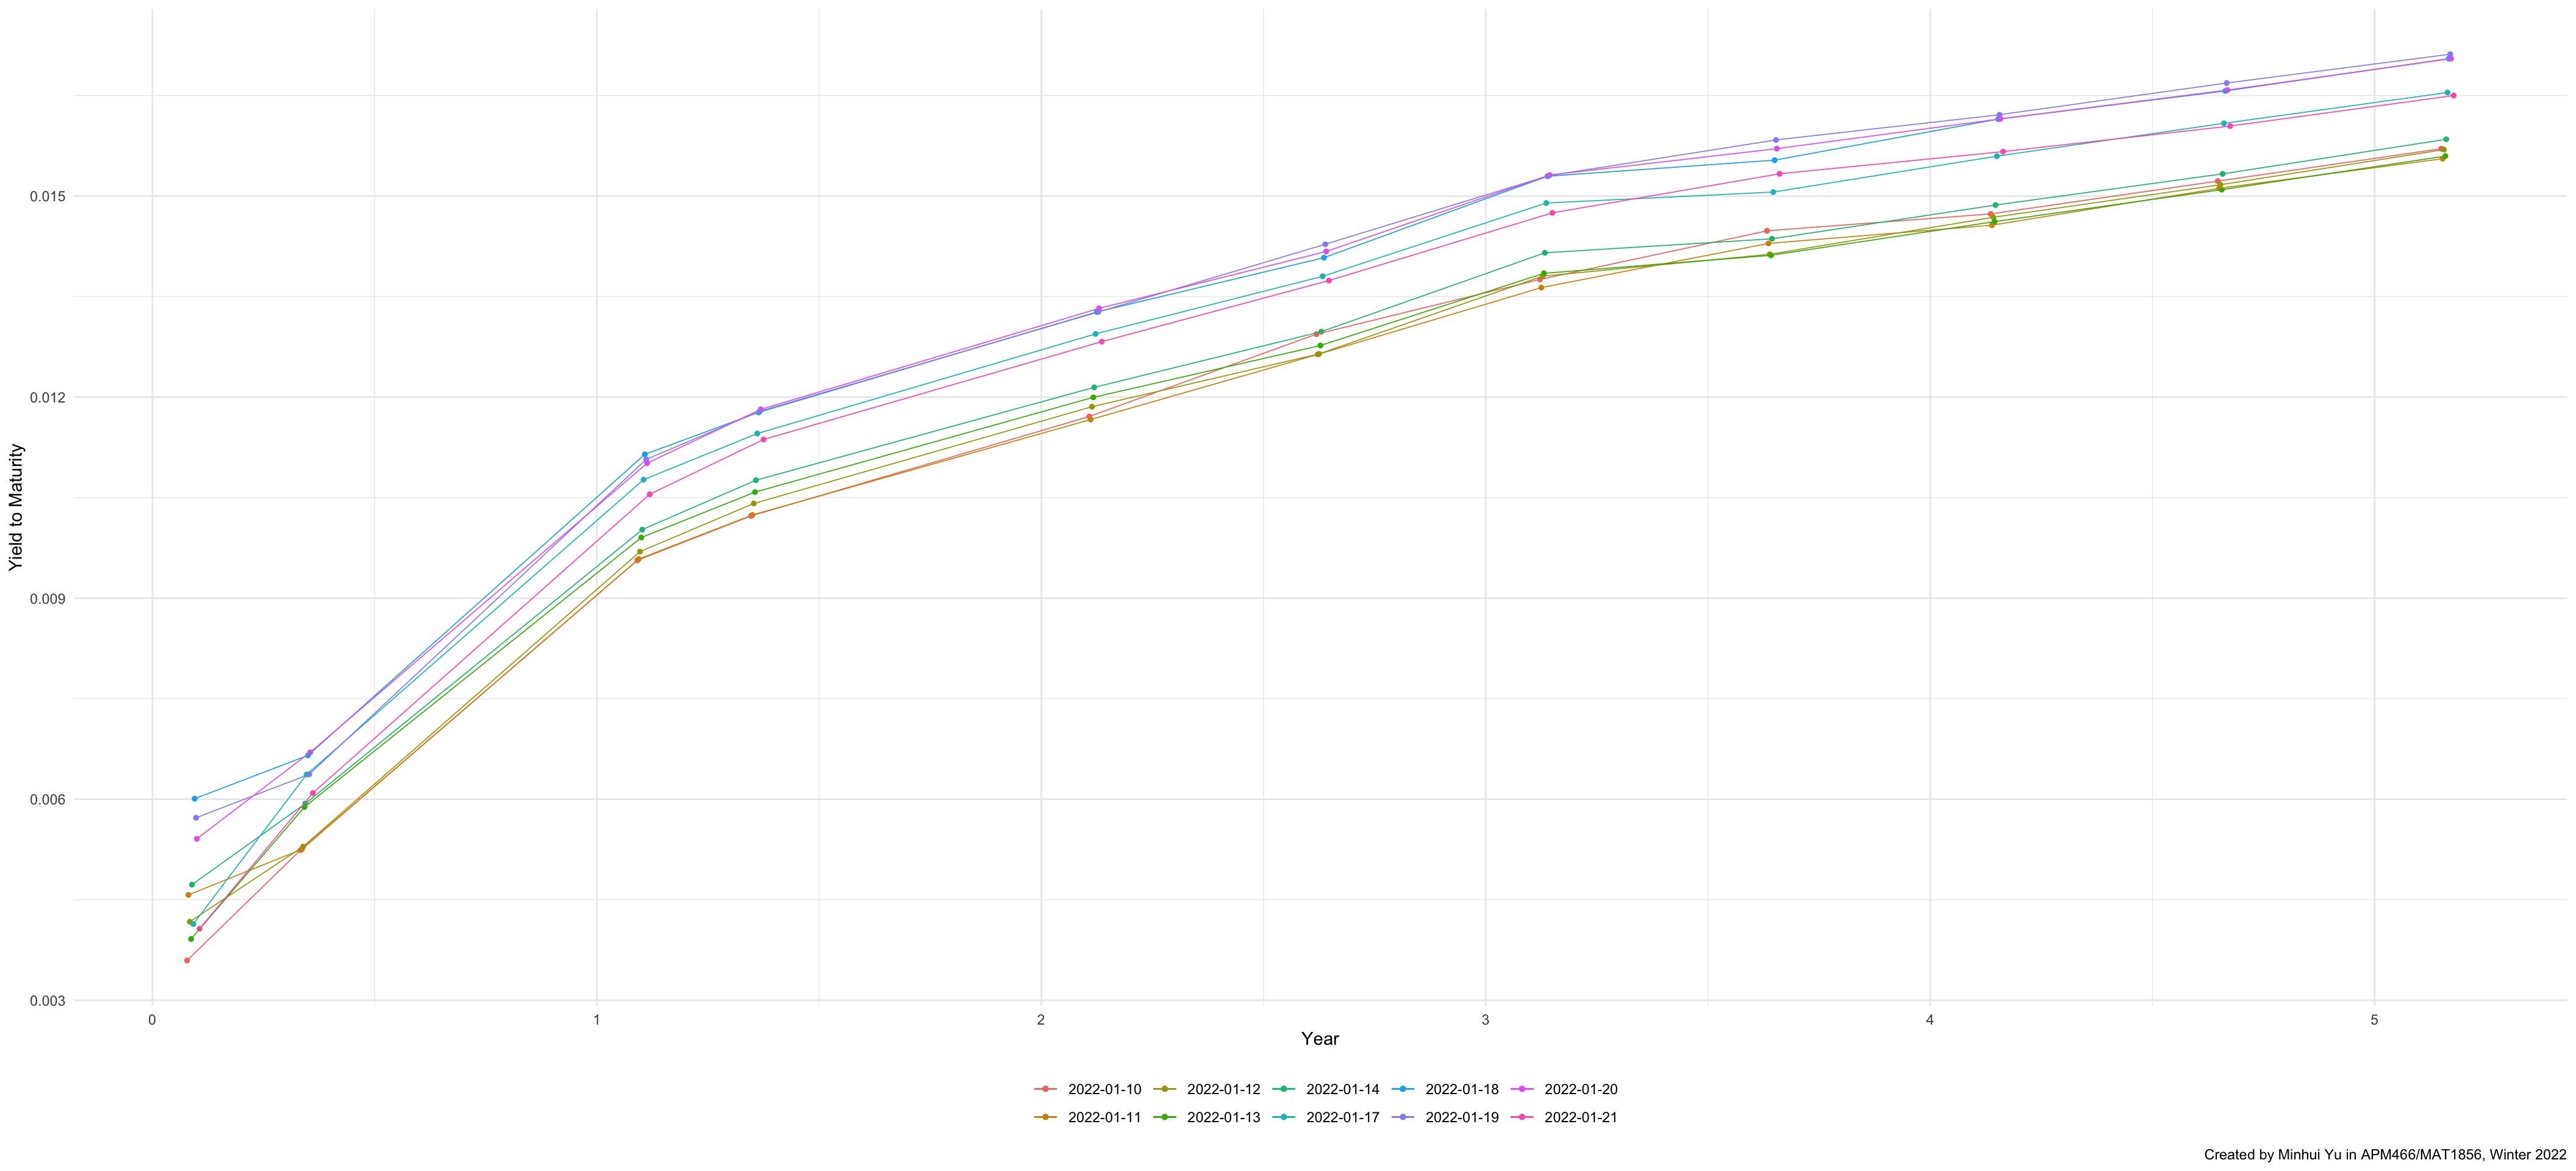
\includegraphics[width=0.7\textwidth]{yield curve.png}
                \caption{5-Year Yield Curve for the Selected 11 Bonds}
            \end{figure}
            The x axis is year and y axis is yield to maturity. There are 10 curves in figure 1 and each stands for one date with identified color. Each line has the similar tendency -- may growing with decreasing growth rate with the shape of the curve seems to convex upward. (we couldn't know for sure, and it need more analysis.)\\
            Interpolation: We need to use exactly 1-year yield in Q5 and Q6 and we only have ytm for approximately years until maturity: 1.2, 2.2, 3.2, 4.2 and 5.2, thus I choose to fit 10 linear regression models based on the data collected date. (Note: Linear regression model may not be the best fitted model for the data, however, since we do not have too much data (11 data in one model), the estimated ytms could be closed to the real ones.) From the summary table, we observed that p-value < 0.05 for both $\beta_0$ and $\beta_1$. Thus there exists significant difference, and we need to reject $H_0: \beta_0 = 0$ and  $H_0: \beta_1 = 0$. So from the linear regression models, we predicted ytm with years until maturity: 1, 2, 3, 4, and 5 in each date, which is shown in table 2.
            \begin{table}[H]
                \caption{Bonds’ Yield (YTM) with Maturity 1-5}
                \resizebox{\textwidth}{9mm}{
                \begin{tabular}{|c|c|c|c|c|c|c|c|c|c|c|} \hline
                    Years Until Maturity & 2022/01/10  & 2022/01/11  & 2022/01/12  & 2022/01/13  & 2022/01/14  & 2022/01/17  & 2022/01/18  & 2022/01/19  & 2022/01/20  & 2022/01/21 \\\hline
                    1 & 0.0081 & 0.0083 & 0.0083 & 0.0084 & 0.0087 & 0.0090 & 0.0097 & 0.0096 & 0.0096 & 0.0090 \\\hline
                    2 & 0.0103 & 0.0104 & 0.0104 & 0.0105 & 0.0107 & 0.0112 & 0.0118 & 0.0118 & 0.0118 & 0.0111 \\\hline
                    3 & 0.0125 & 0.0124 & 0.0125 & 0.0125 & 0.0128 & 0.0134 & 0.0139 & 0.0139 & 0.0139 & 0.0133 \\\hline
                    4 & 0.0147 & 0.0145 & 0.0146 & 0.0146 & 0.0148 & 0.0156 & 0.0160 & 0.0161 & 0.0160 & 0.0156 \\\hline
                    5 & 0.0169 & 0.0166 & 0.0167 & 0.01667 & 0.0169 & 0.0178 & 0.0181 & 0.0183 & 0.0182 & 0.0178 \\\hline
                \end{tabular}}
            \end{table}
        \item 
            Recall: $P_n = \sum_{i = 1}^{n} {{cash \ flow_i} \times (1 + \frac{r_i}{2})^{-2 t_i}}$, where $n \in [1, 11]$, where $r_i$ is the spot rate, $P_i$ is the dirty price and $t_i$ is the years until maturity. The difference between calculating YTM and spot rate is YTM has same r for one equation while spot rate has different r. \\
            The pseudo-code for calculating spot rate: \\
            Recall time\_interval is a vector with elements 0.5-1, 1-1.5, \dots, 4.5-5 and 5+ year; dates is a vector with elements 2022/01/10 - 2022/01/14 and 2022/01/17 - 2022/01/21; years\_until\_maturity is a 11 $\times$ 10 matrix, and years\_until\_maturity[i,j] represents the years until maturity for $i^{th}$ date and $j^{th}$ bond in data; cash\_flow is a 11$\times$11 matrix and cash\_flow[i,j] represents the cash flow for $i^{th}$ bond in $j^{th}$ year interval.
            
            $$
            \begin{scriptsize}
            \begin{aligned}
            & let \ spot\_rate \ be \ a \ new \ 11 \times 10 \ matrix \ with \ all \ original \ elements \ are \ 0 \\
            & let \ the \ row \ name \ of \ spot\_rate \ be \ time\_interval \\
            & let \ the \ column \ name \ of \ spot\_rate \ be \ dates \\
            & for \ i \ in \ the \ range \ of \ \# \ of \ row \\
            & \qquad for \ j \ in \ the \ range \ of \ \# \ of \ column \\
            & \qquad \qquad there \ are \ 11 \ cases \ in \ total \\
            & \qquad \qquad if \ i == 1 \ and \ i == 2 \\
            & \qquad \qquad \qquad // \ since \  years\_until\_maturity[2,j] < 0.5 \\
            & \qquad \qquad \qquad // \ so \ spot\_rate[1,j] \ and \ spot\_rate[2,j] will \ be \ calculated \ by \ the \ same method \\
            & \qquad \qquad \qquad spot\_rate[i,j] \leftarrow ytm[i,j] \\
            & \qquad \qquad else \ if \ i == 3 \\
            & \qquad \qquad \qquad let \ f(r) = cash\_flow[i,1]*(1 + spot\_rate[1, j]/2)^{-years\_until\_maturity[1,j]*2} \\
            & \qquad \qquad \qquad \qquad \quad - cash\_flow[i,2]*(1 + spot\_rate[2,j]/2)^{-years\_until\_maturity[2,j]*2} \\
            & \qquad \qquad \qquad \qquad \quad -cash\_flow[i,3]*(1 + r/2)^{- years\_until\_maturity[3,j] * 2} \\
            & \qquad \qquad \qquad spot\_rate[i,j] \leftarrow uniroot(f(r), c(0,1))\$root \\
            & \qquad \qquad else \ if \ i == 4 \\
            & \qquad \qquad \qquad // \ since \  years\_until\_maturity[4,j] < 1.5 \\
            & \qquad \qquad \qquad // \ so \ spot\_rate[3,j] \ and \ spot\_rate[4,j] will \ be \ calculated \ by \ the \ same method \\
            & \qquad \qquad \qquad let \ f(r) = cash\_flow[i,1]*(1 + spot\_rate[1, j]/2)^{-years\_until\_maturity[1,j]*2} \\
            & \qquad \qquad \qquad \qquad \quad - cash\_flow[i,2]*(1 + spot\_rate[2,j]/2)^{-years\_until\_maturity[2,j]*2} \\
            & \qquad \qquad \qquad \qquad \quad -cash\_flow[i,3]*(1 + r/2)^{- years\_until\_maturity[4,j] * 2} \\
            & \qquad \qquad \qquad spot\_rate[i,j] \leftarrow uniroot(f(r), c(0,1))\$root \\
            & \qquad \qquad // \ r \ in \ the \ remaining \ cases \ is \ consistent \ with \ the \ calculation \ method \ of \ r \ in \ case \ i == 3 \\
            & \qquad \qquad else \ if \ i == 5 \\
            & \qquad \qquad \vdots \\
            & \qquad \qquad \vdots \\
            & \qquad \qquad else \ if \ i == 11 \\
            & \qquad \qquad \qquad \cdots \\
            & // \ now \ we \ are \ done \ for \ calculated \ spot \ rate 
            \end{aligned}
            \end{scriptsize}
            $$ 
            
            And here is the plot for spot rate: 
            \begin{figure}[H]
                \centering
                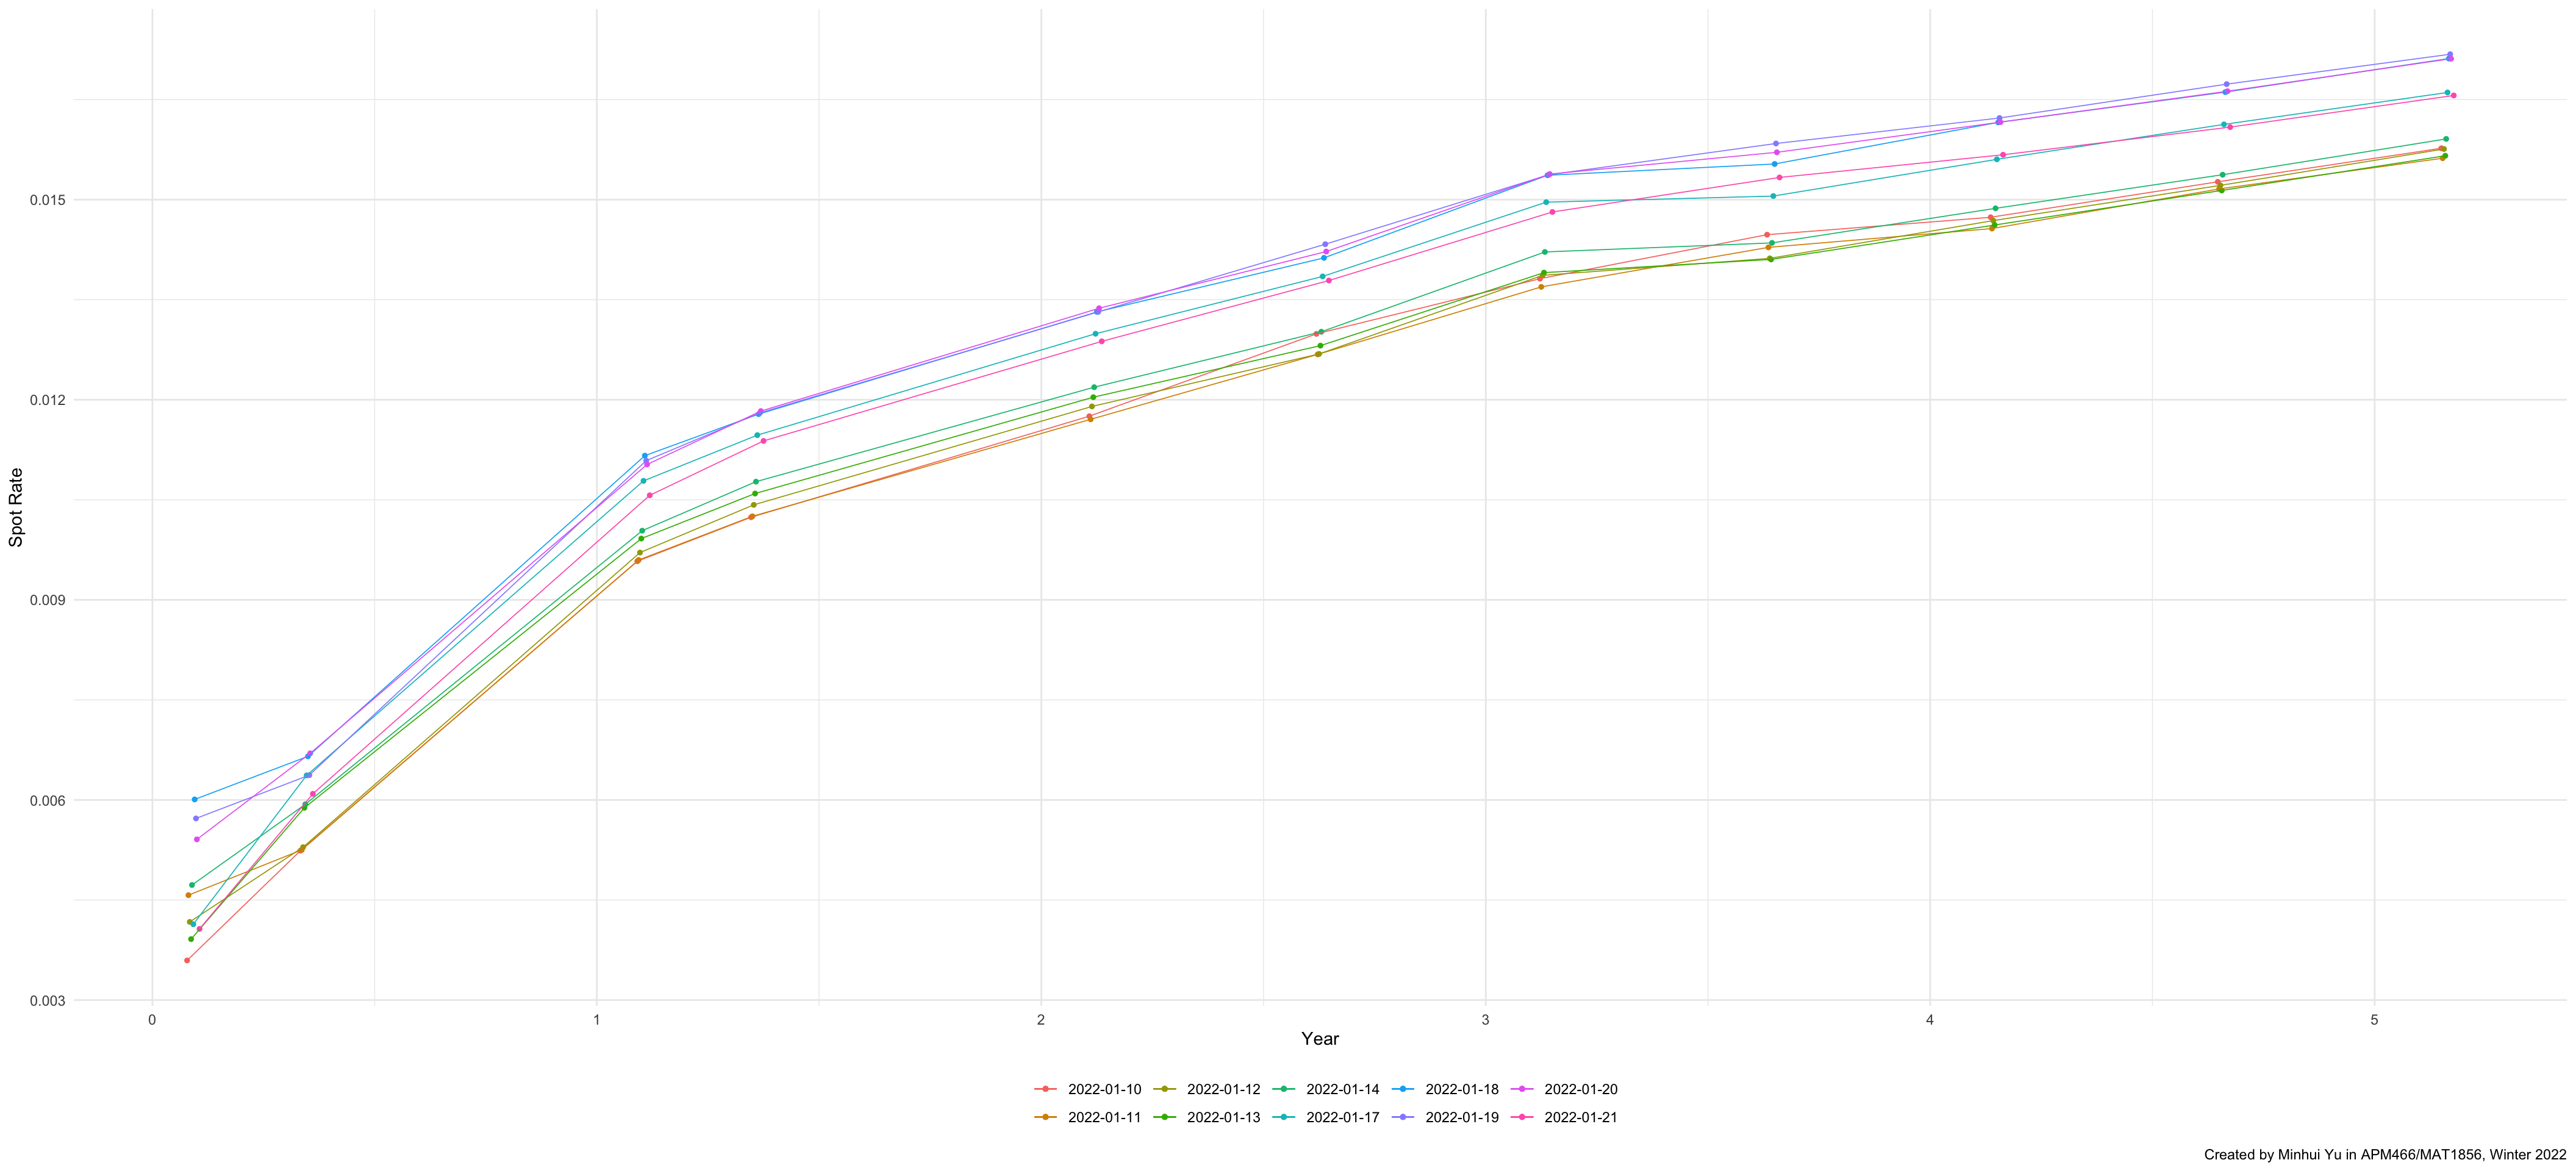
\includegraphics[width=0.7\textwidth]{spot rate curve.png}
                \caption{5-Year Spot Rate Curve for the Selected 11 Bonds}
            \end{figure}
            The spot rate curves is very similar to the bond's yield curves. They both have years on the x axis, and the y axis of the spot rate curve is the spot rate. The reason is that spot rate is also known as the zero interest rate which means we find it by discount the cash flow and discount rate is what we need.
        \item 
            For forward rate we have the equation below, where t represents the years until maturity and $s_t$ represents the spot rate with years until maturity t, $f_{1yr, \ iyr}$ represents the forward rate starting in one year and going i more years where i $\in$ \{1, 2, 3, 4\}. The reason why I choose spot\_rate[3,j] is the years until maturity of spot\_rate[2,j] is about 0.333 while the years until maturity of spot\_rate[3,j] is about 1.1 which is more closer to 1 year.
            $$
            \begin{scriptsize}
            \begin{aligned}
            \qquad (1 + \frac{f_{t-i,\ t}}{2})^{t-(t-i)} = \frac{(1+s_t)^t}{(1+s_{t-i})^{t-i}} & \Rightarrow f_{t-i,\ t} = 2 \times \left[ \sqrt[i]{\frac{(1+s_t)^t}{(1+s_{t-i})^{t-i}}} - 1 \right] \\
            (focus \ on \ the \ data \ in \ one \ date) & \Rightarrow f_{1yr-iyr} = f_{3,\ 2i + 1} = 2 \times \left[ \sqrt[2i-2]{\frac{(1+s_{2i + 1})^{2i + 1}}{(1+s_{3})^{3}}} - 1 \right]
            \end{aligned}
            \end{scriptsize}
            $$
            The pseudo-code for calculating forward rate: 
            $$
            \begin{scriptsize}
            \begin{aligned}
            & let \ forward\_rate \ be \ a \ new \ 4 \times 10 \ matrix \ with \ all \ original \ elements \ are \ 0 \\
            & let \ f\_time\_interval \ be \ a \ vector \ with \ given \ year \ interval \ inside \\
            & // \ given \ year \ interval \ are \ 1yr-1yr, \ 1yr-2yr, \ 1yr-3yr, \ and \ 1yr-4yr \\
            & let \ the \ row \ name \ of \ forward\_rate \ be \ f\_time\_interval \\
            & let \ the \ column \ name \ of \ forward\_rate \ be \ dates \\
            & for \ i \ in \ the \ range \ of \ \# \ of \ row \\
            & \qquad for \ j \ in \ the \ range \ of \ \# \ of \ column \\
            & \qquad \qquad let \ forward\_rate[i,j] \leftarrow 2*(((1+spot\_rate[2(i+1)+1,j]/2)^{years\_until\_maturity[(i+1)*2+1,j]} \\
            & \qquad \qquad \qquad \qquad \qquad \qquad \qquad \qquad /(1+spot\_rate[3,j]/2)^{years\_until\_maturity[3,j]}) \\ 
            & \qquad \qquad \qquad \qquad \qquad \qquad \qquad \qquad ^{(1/(years\_until\_maturity[2(i+1)+1,j] -years\_until\_maturity[3,j]))} -1) \\
            & // \ now \ we \ are \ done \ for \ calculated \ forward \ rate 
            \end{aligned}
            \end{scriptsize}
            $$
            And here is the plot for forward rate: 
            \begin{figure}[H]
                \centering
                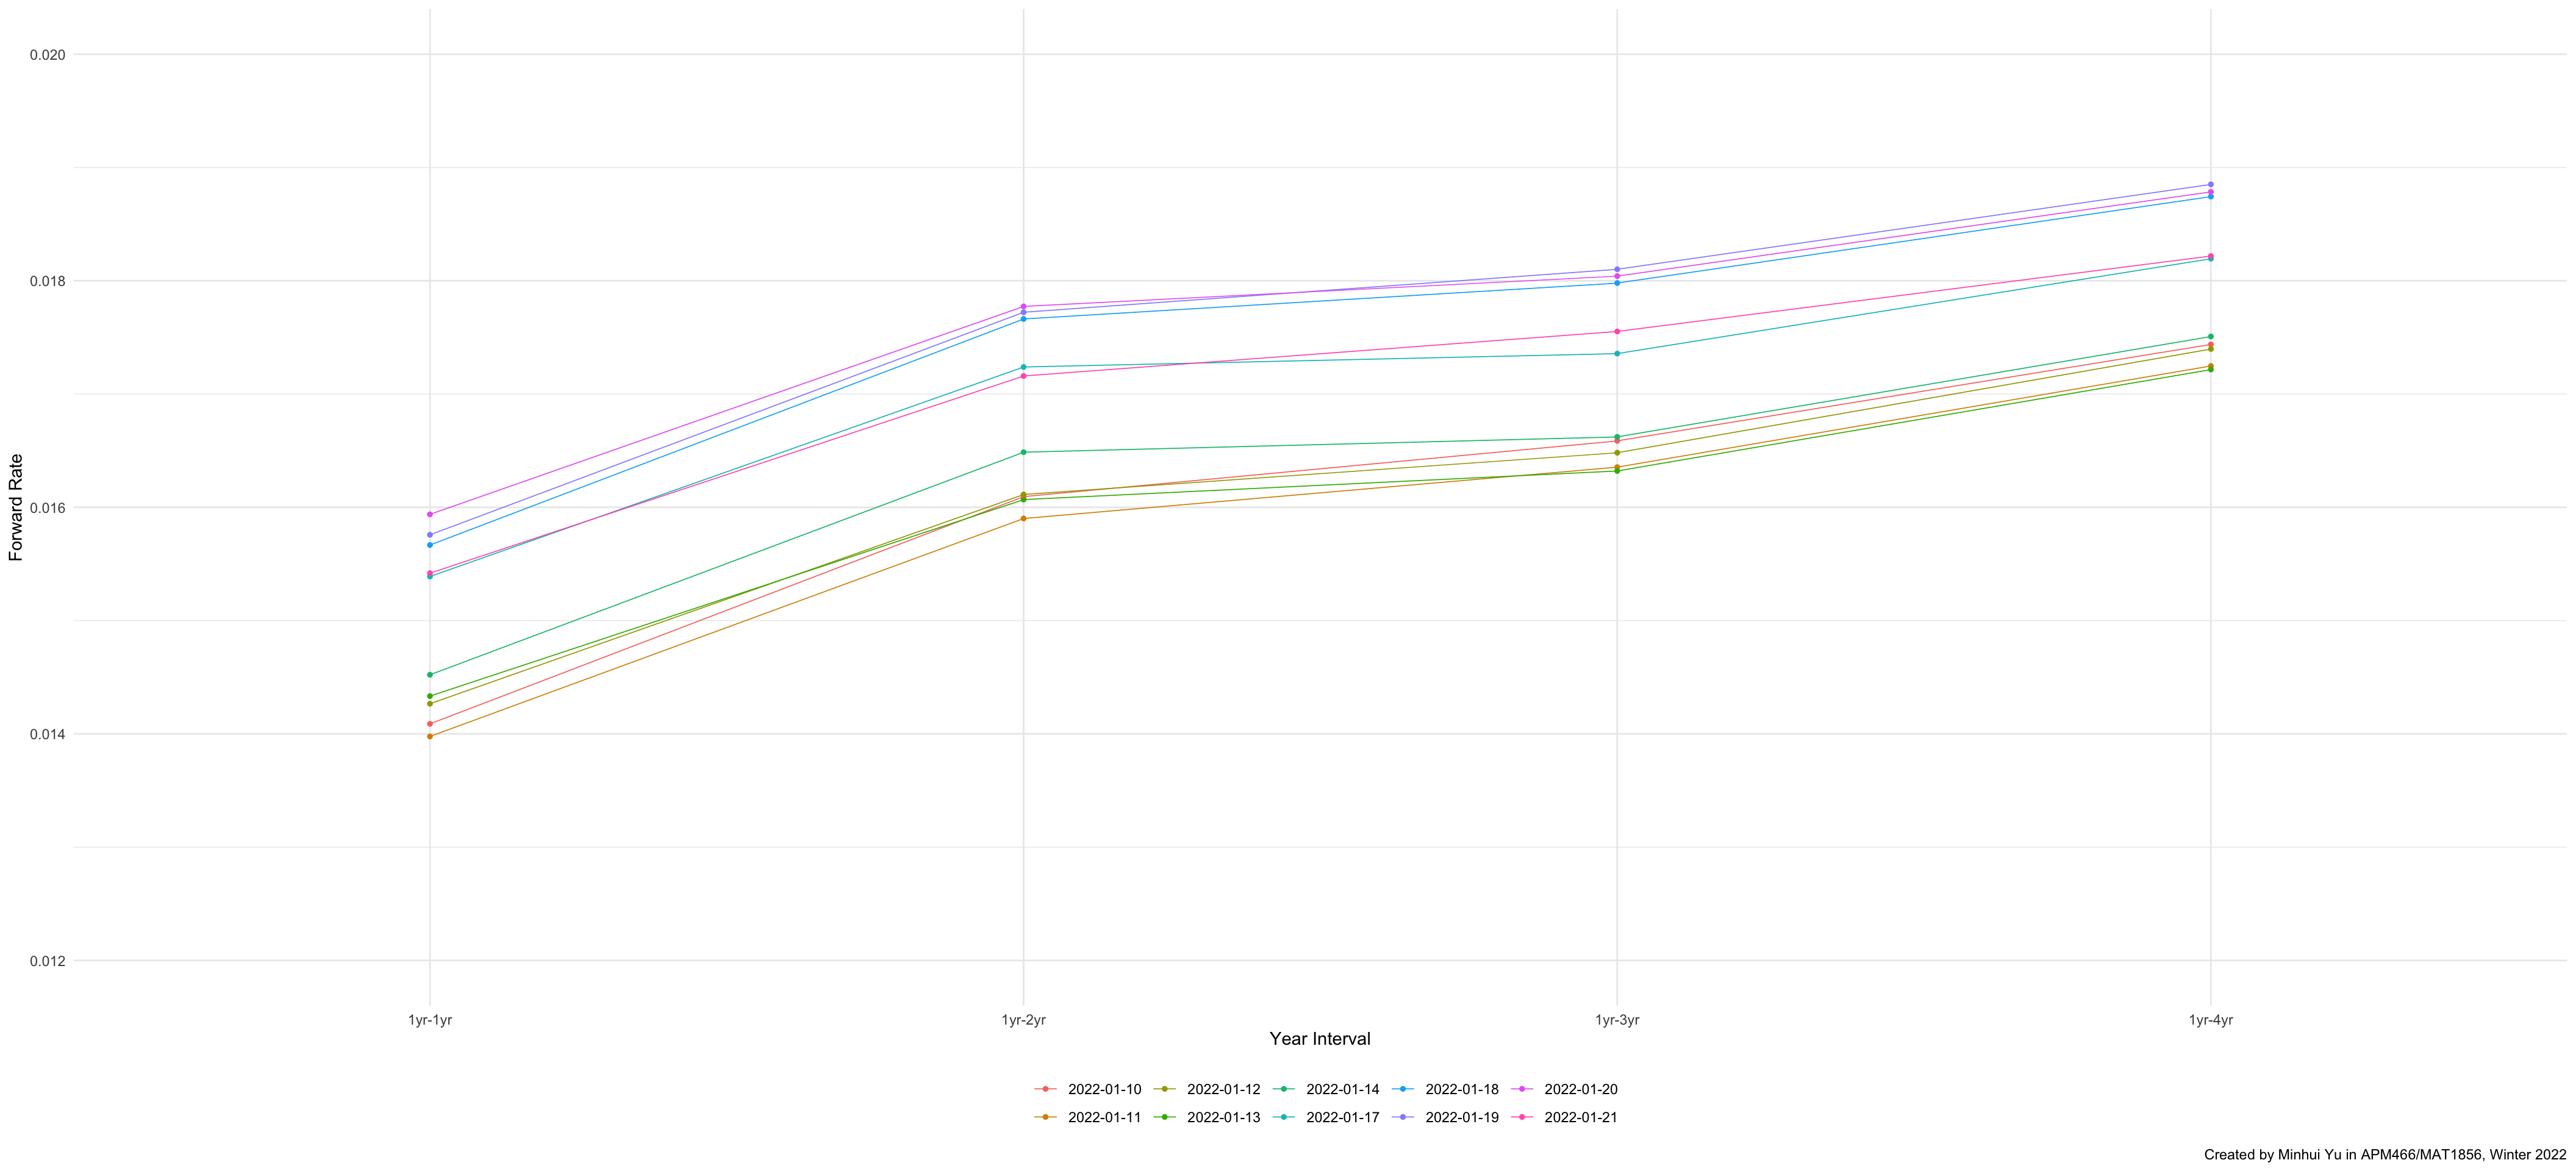
\includegraphics[width=0.7\textwidth]{forward rate curve.png}
                \caption{5-Year Spot Rate Curve for the Selected 11 Bonds}
            \end{figure}
            The x axis is time interval  1yr-1yr, 1yr-2yr, 1yr-3yr, and 1yr-4yr and the y axis is forward rate. There are 10 curves in figure 1 and each stands for one date with identified color. Most curve shows that the forward rate will increase for long time interval. Note that the forward rate here from derivation is implicit and does not represent the market's expectation of forward rate.
    \end{enumerate}
        
    \item 
        Let $C_1$  =  Cov(log-return of yield) and $C_2$ = Cov(log-return of forward rate). Since log-return of yield is calculated by yield in table 2 above which has 5 year's yield, then log-return of yield is a 9 $\times$ 5 matrix where 10 represents there are 9 $day_i$-$day_{i+1}$ differences with 10 date in original and 5 represents 1-year, 2-year, \dots, 5-year time series. Similarly, log-return of forward rate is a 9 $\times$ 4 matrix with 4 year interval as the same in Q4.(c). Since we focus on times series for both daily return-log yield and forward rate, then when we calculate the covariance of them respectively based on the formula: $cov\left( \sum_{i=1}^n X_i, \ \sum_{i=1}^n X_i \right) = var\left( \sum_{i=1}^n X_i \right)$ where $X_i$ has a time series $X_{i,\ j} = \log(r_{i, \ j+1} / r_{i, \ j})$. And based on the discussion above, n = 5 for $C_1$ and n = 4 for $C_2$, j $\in$ \{1, 2, \dots, 9\}. The time series $X_{i, \ j}$ is essentially the rate of return on the term as it compounds to infinity and logarithms are additive. So $X_{i, \ j}$ represents the log difference between rate $r_{i, \ j+1}$ and $r_{i, \ j}$ and it can also eliminate part of the linear influence ( degree of independent) between  $r_{i, \ j+1}$ and $r_{i, \ j}$ -- the covariance became smaller.
        $$
        \begin{scriptsize}
            \begin{array}{ll}
            C_1 = \begin{pmatrix}
            0.00169 & 0.00125 & 0.00095 & 0.00073 & 0.00057 \\
            0.00125 & 0.00097 & 0.00078 & 0.00065 & 0.00054 \\
            0.00095 & 0.00078 & 0.00067 & 0.00059 & 0.00052 \\
            0.00073 & 0.00065 & 0.00059 & 0.00054 & 0.00051 \\
            0.00057 & 0.00054 & 0.00052 & 0.00051 & 0.00050
            \end{pmatrix},
            \ C_2 = \begin{pmatrix}
            0.00059 & 0.00054 & 0.00049 & 0.00047 \\
            0.00054 & 0.00055 & 0.00052 & 0.00049 \\
            0.00049 & 0.00052 & 0.00053 & 0.00049 \\
            0.00047 & 0.00049 & 0.00049 & 0.00046
            \end{pmatrix}
            \end{array}
        \end{scriptsize}
        $$
    \item
        $\lambda_{y_1}$ is corresponding to $\xi_{y_1}$. $\lambda_{y_1}$ is the variance of the corresponding dimension of the data after transformation and implies the contribution of $\xi_{y_1}$ to the covariance matrix of log-return yield with percentage $\lambda_{y_1} \sum_{i = 1}^5 \lambda_{y_i}$. $\xi_{y_1}$ implies the direction of change in yield., which is in the wave.
        $$
        \begin{scriptsize}
            \begin{array}{ll}
            \begin{pmatrix} 
            \lambda_{y_1} \\ 
            \lambda_{y_2} \\
            \lambda_{y_3} \\        
            \lambda_{y_4} \\
            \lambda_{y_5} \\
            \end{pmatrix} = \begin{pmatrix}
            3.9616 \times 10^{-3}  \\
            4.1833 \times 10^{-4} \\
            3.2897 \times 10^{-8} \\
            1.0236 \times 10^{-12} \\
            6.7514 \times 10^{-18}
            \end{pmatrix}, \quad
            \begin{pmatrix} 
            \xi_{y_1}, & 
            \xi_{y_2}, &
            \xi_{y_3}, &        
            \xi_{y_4}, &
            \xi_{y_5} 
            \end{pmatrix} = \begin{pmatrix}
            0.625 &  0.590 & -0.480 & -0.173 & -0.033 \\
            0.495 &  0.108 & 0.534 & 0.628 & 0.252 \\
            0.405 & -0.216 & 0.454 & -0.409 & -0.645 \\
            0.340 & -0.450 & 0.015 & -0.475 & 0.676 \\
            0.291 & -0.626 & -0.527 & 0.428 & -0.250
            \end{pmatrix}
            \end{array}
        \end{scriptsize}
        $$
        $$
        \begin{scriptsize}
            \begin{array}{ll}   
            \begin{pmatrix} 
            \lambda_{f_1} \\ 
            \lambda_{f_2} \\
            \lambda_{f_3} \\        
            \lambda_{f_4} 
            \end{pmatrix} = \begin{pmatrix}
            2.0363 \times 10^{-3}  \\
            8.1254 \times 10^{-5} \\
            1.3659 \times 10^{-5} \\
            1.7300 \times 10^{-6}
            \end{pmatrix}, \quad
            \begin{pmatrix} 
            \xi_{f_1}, & 
            \xi_{f_2}, &
            \xi_{f_3}, &       
            \xi_{f_4} 
            \end{pmatrix}= \begin{pmatrix}
            -0.514 & 0.782 & 0.352 & 0.006 \\
            -0.513 & 0.042 & -0.841 & -0.166 \\
            -0.500 & -0.502 & 0.395 & -0.585 \\
            -0.472 & -0.366 & 0.113 & 0.794
            \end{pmatrix}
            \end{array}
        \end{scriptsize}
        $$
        
\end{enumerate}

\subsection*{References}

$[1]$ Latex mathematical Formulas. "Latex mathematical Formulas - detailed tutorial" Published October 2020.\\
\href{https://blog.csdn.net/NSJim/article/details/109045914} {https://blog.csdn.net/NSJim/article/details/109045914} \\
$[2]$ Rpubs.com. 2022. RPubs - Bond Valuation and Analysis in R. Accessed 14 February 2022. \\ \hrec{https://rpubs.com/Sergio_Garcia/bond_valuation_analysis_r}{https://rpubs.com/Sergio_Garcia/bond_valuation_analysis_r} \\
$[3]$ Oeis.org. 2019. List of LaTeX mathematical symbols - OeisWiki. Accessed 14 February. \\ \href{https://oeis.org/wiki/List_of_LaTeX_mathematical_symbols_2022}{https://oeis.org/wiki/List_of_LaTeX_mathematical_symbols}.

\subsection*{GitHub Link to Code}

\href{https://github.com/minhui-yu-helen/APM466H1-Assignment-1}{https://github.com/minhui-yu-helen/APM466H1-Assignment-1}

\end{document}
